%% ****** Start of file aiptemplate.tex ****** %
%%
%%   This file is part of the files in the distribution of AIP substyles for REVTeX4.
%%   Version 4.1 of 9 October 2009.
%%
%
% This is a template for producing documents for use with 
% the REVTEX 4.1 document class and the AIP substyles.
% 
% Copy this file to another name and then work on that file.
% That way, you always have this original template file to use.

\documentclass[%
 prl,
% jmp,
% bmf,
% sd,
% rsi,
 amsmath,amssymb,
%
 reprint,%
%author-year,%
%author-numerical,%
% Conference Proceedings
]{revtex4-1}

\usepackage{graphicx}% Include figure files
\usepackage{dcolumn}% Align table columns on decimal point
\usepackage{bm}% bold math
%\usepackage[mathlines]{lineno}% Enable numbering of text and display math
%\linenumbers\relax % Commence numbering lines

\usepackage[utf8]{inputenc}
\usepackage[T1]{fontenc}
\usepackage{mathptmx}
\usepackage{etoolbox}

%%%%%%%%%%%%%%%%%% makes hyperlinks work %%%%%%%%%%%%%%%%%%%%%%%%%%%%%%%%%
\usepackage{xcolor,hyperref}
\hypersetup{
   colorlinks,
   linkcolor={blue!50!black},%{red!80!black},
   citecolor={blue!50!black},
   urlcolor={blue!80!black}
}
%%%%%%%%%%%%%%%%%%%%%%%%%%%%%%  END %%%%%%%%%%%%%%%%%%%%%%%%%%%%%%%%%%%%%%%
%% Apr 2021: AIP requests that the corresponding 
%% email to be moved after the affiliations
\makeatletter
\def\@email#1#2{%
 \endgroup
 \patchcmd{\titleblock@produce}
  {\frontmatter@RRAPformat}
  {\frontmatter@RRAPformat{\produce@RRAP{*#1\href{mailto:#2}{#2}}}\frontmatter@RRAPformat}
  {}{}
}%
\makeatother

\draft % marks overfull lines with a black rule on the right

\begin{document}

% Use the \preprint command to place your local institutional report number 
% on the title page in preprint mode.
% Multiple \preprint commands are allowed.
%\preprint{}

\title{Anomalous softness in amorphous matter in the reversible plastic regime} %Title of paper

% repeat the \author .. \affiliation  etc. as needed
% \email, \thanks, \homepage, \altaffiliation all apply to the current author.
% Explanatory text should go in the []'s, 
% actual e-mail address or url should go in the {}'s for \email and \homepage.
% Please use the appropriate macro for the type of information

% \affiliation command applies to all authors since the last \affiliation command. 
% The \affiliation command should follow the other information.

\author{A.~Elgailani}
\affiliation{Northeastern University, Boston, Massachusetts 02115, USA}
\author{D.~Vandembroucq}
\affiliation{PMMH, CNRS UMR 7636, ESPCI Paris, PSL University, Sorbonne  Université, Université  de Paris, F-75005 Paris, France}
\author{C.E. ~Maloney}
\affiliation{Northeastern University, Boston, Massachusetts 02115, USA}

% Collaboration name, if desired (requires use of superscriptaddress option in \documentclass). 
% \noaffiliation is required (may also be used with the \author command).
%\collaboration{}
%\noaffiliation

\date{\today}

\begin{abstract}
We study an integer automaton elasto-plastic model of an amorphous solid subject to cyclic shear of amplitude $\Gamma$.
We focus on the reversible plastic regime (RPR) at intermediate $\Gamma$, where, after a transient, the system settles into a periodic limit cycle with dissipative plastic events which, although they lead to hysteresis, precisely reverse themselves microscopically after an integer number of loading cycles.
We study the plastic strain rate, $\frac{d\epsilon}{d\gamma}$, (where $\gamma$ is the applied strain and $\epsilon$ is the resulting plastic strain) during the terminal limit cycles and show that it consists of a creeping regime at low $\gamma$ with very low $\frac{d\epsilon}{d\gamma}$ followed by a sharp transition at a characteristic strain, $\gamma_*$, and stress, $\sigma_*$ to a flowing regime at higher $\frac{d\epsilon}{d\gamma}$.
We show that while increasing $\Gamma$ results in lower terminal ground state energy, $E_{\text{min}}$, it, surprisingly, results in \emph{lower} $\gamma_*$, and $\sigma_*$.
In this sense, the lower energy states obtained at higher cycling amplitude are, counter-intuitively, softer than the higher energy states obtained at lower cycling amplitude.
We relate this anomalous softness to an emergent characteristic feature in the stress distribution, $P(\sigma)$, at a value, $\sigma^\dagger$, which is independent of $\Gamma$ and show that $\sigma^\dagger$ implies a relation between the $\Gamma$ dependence of $\sigma_*$, $\gamma_*$, and the amplitude of plastic strain, $\Delta\epsilon$, and energy dissipation, $\Delta U$.
Our results place important constraints on mean-field theories of amorphous matter and should motivate experiments on cyclically sheared systems such as amorphous alloys, colloidal glasses, emulsions, pastes, granular matter, etc.
\end{abstract}

\pacs{}% insert suggested PACS numbers in braces on next line

\maketitle %\maketitle must follow title, authors, abstract and \pacs

% Body of paper goes here. Use proper sectioning commands.
\section{\label{sec:intro} Introduction}
There is a huge variety of non-crystalline solids including foams, pastes, emulsions, metallic alloys, glassy polymers, colloidal glasses, dense granular matter, etc. each of which exhibits a similar phenomenology when subjected to shear. 
Recent work has focused on the response to cyclic shear in the forward and reverse sense, where the material is sheared in forward and backward along a single direction of shear.  
Cyclic shearing experiments have been performed on foams~\cite{Dennis-Ohern}, and emulsion~\cite{Cloitre,PineCipilletti},  but perhaps the clearest and most precise and informative experiments have been performed by Keim and co-workers on 2D rafts of polystyrene particles trapped at an oil-water interface.
In those experiments, it was shown that, depending on the shearing amplitude, $\Gamma$, one reaches one of three terminal steady state behaviors.
At the lowest $\Gamma$, after a transient, the system responds completely elastically with no rearrangements or any kind of energy dissipating events at all.
We refer to this as the elastic regime (ER).
At higher $\Gamma$, rearrangements — along with their associated energy dissipation and hysteresis — occur, but the rearrangements precisely reverse themselves microscopically after one or more shear cycles.
The system remains trapped within a finite set of microscopic configurations and there is no long time diffusive behavior despite the hysteresis and energy dissipation during the shear cycles.
We refer to this as the reversible plastic regime (RPR).
Finally, at the highest $\Gamma$, the system never returns to a previous configuration even after an arbitrarily large number of shear cycles, and the long-time behavior is diffusive.
We refer to this regime as the diffusive regime (DR).
The reversible plastic regime has also been identified in atomistic~\cite{ohern-denin, Regev} and elasto-plastic~\cite{kareem, muhitin-etal} models.
There is currently some confusion and no consensus in the community as to which of the two transitions, ER->RPR or RPR->DR should be considered the “yielding transition” and, to the extent that other authors are even clear about which of the two transitions they focus on, the nature and order of the transitions are still a matter of debate.

Here, we study a simple elasto-plastic integer automaton model (EPM) for an amorphous solid subjected to cyclic shear in the athermal, quasi static (AQS) limit.  
The model is described in detail below, but the important feature which distinguishes it from other related EPMs is that we introduce no disorder or stochasticity into the model after an initial quench protocol.
This allows our EPM to capture the reversible trajectories in the RPR regime seen in particle-based simulations (\cite{Regev}) and experiments (\cite{Ohern,Keim}). 
We also focus exclusively on initial states which are maximally disordered and correspond to rapidly quenched glasses or violently prepared emulsions/foams/colloidal glasses or amorphous allows with little thermal relaxation allowed before the initiation of cyclic shearing, whereas other studies~\cite{Muhitin,Kirsten,Sastry} have focused on the behavior of systems with different thermal annealing histories or different quench protocols.

In our EPM, we have an additive decomposition of the strain into an elastic and plastic contribution so that $\sigma=\mu (\gamma-\epsilon)$ where $\sigma$ is the total shear stress, $\gamma$ is the imposed strain, and $\epsilon$ is the plastic strain in the material.
$\mu$ is the elastic shear modulus, and we measure all stresses in this work in units of $\mu$, so we simply have: $\sigma=\gamma-\epsilon$.
Our primary goal is to characterize the behavior of the limit cycles in the RPR, but we also study the transition between the ER and the RPR and show that it has a mixed character between first and second order.
We note that even though the final steady states in the ER are trivial and devoid of any plastic relaxation, the ground state energy (the energy of the stress-free configuration visited during a shear cycle) decreases with each successive cycle until the plasticity vanishes, so the terminal ground state energy is a non-trivial function of $\Gamma$, even in the ER.  
If we characterize the system via the value of the ground state energy, the ER->RPR transition is completely invisible!
A similar characterization via the residual strain (defined below) is also completely blind to the ER->RPR transition.
If we characterize the system via the amount of energy dissipated per shear cycle in the terminal steady state or even more simply the amount of plastic strain generated in a strain-sweep, then we have something like a second order transition, where below the ER->RPR transition, there is precisely zero energy dissipated and no plastic strain, but above the transition, the dissipated energy and the plastic strain increase with $\Gamma$ continuously from zero.
Finally, if we look at the behavior of the $\epsilon$ vs $\gamma$ hysteresis curves, above the ER->RPR transition, the plastic strain rate, $\frac{d \epsilon}{d\gamma }$ turns on quite suddenly at a characteristic strain value, $\gamma_*$, and jumps from zero to a finite value of about $0.15$ regardless of the cycling amplitude; reminiscent of a first order transition.
Although the value of the plastic strain rate at the onset of plasticity is insensitive to $\Gamma$, the strain and stress at which plasticity begins, $\gamma_*$ and $\sigma_*$ both \emph{decrease} with increasing $\Gamma$ indicating that the systems which are cycled at higher $\Gamma$ are actually \emph{softer} than those cycled at lower $\Gamma$.
This behavior is striking and counter-intuitive, as one would expect the systems at higher $\Gamma$ to be \emph{harder} given their lower energy and narrower stress distribution…. presumably indicative of a deeper quench.
We also show that the total plastic strain incurred in the cycle, $\epsilon_t$, shows an associated non-trivial increase with $\Gamma$. 
We show that the $\Gamma$ dependence of $\gamma_*$, $\sigma_*$, and $epsilon_t$ can be understood by the emergence of a non-trivial $\Gamma$-\emph{independent} characteristic stress, $\sigma^\dagger$ which is evident in the probability distribution of the stress, $P(\sigma)$, for all systems in the RPR.  


% References should be done using the \cite, \ref, and \label commands
\section{figures}
%\label{}

%%%%%%%%%%%%%%%%%%%%%%%%%%%%%%%% Figure 1 %%%%%%%%%%%%%%%%%%%%%%%%%%%%%
\begin{figure}[h!]
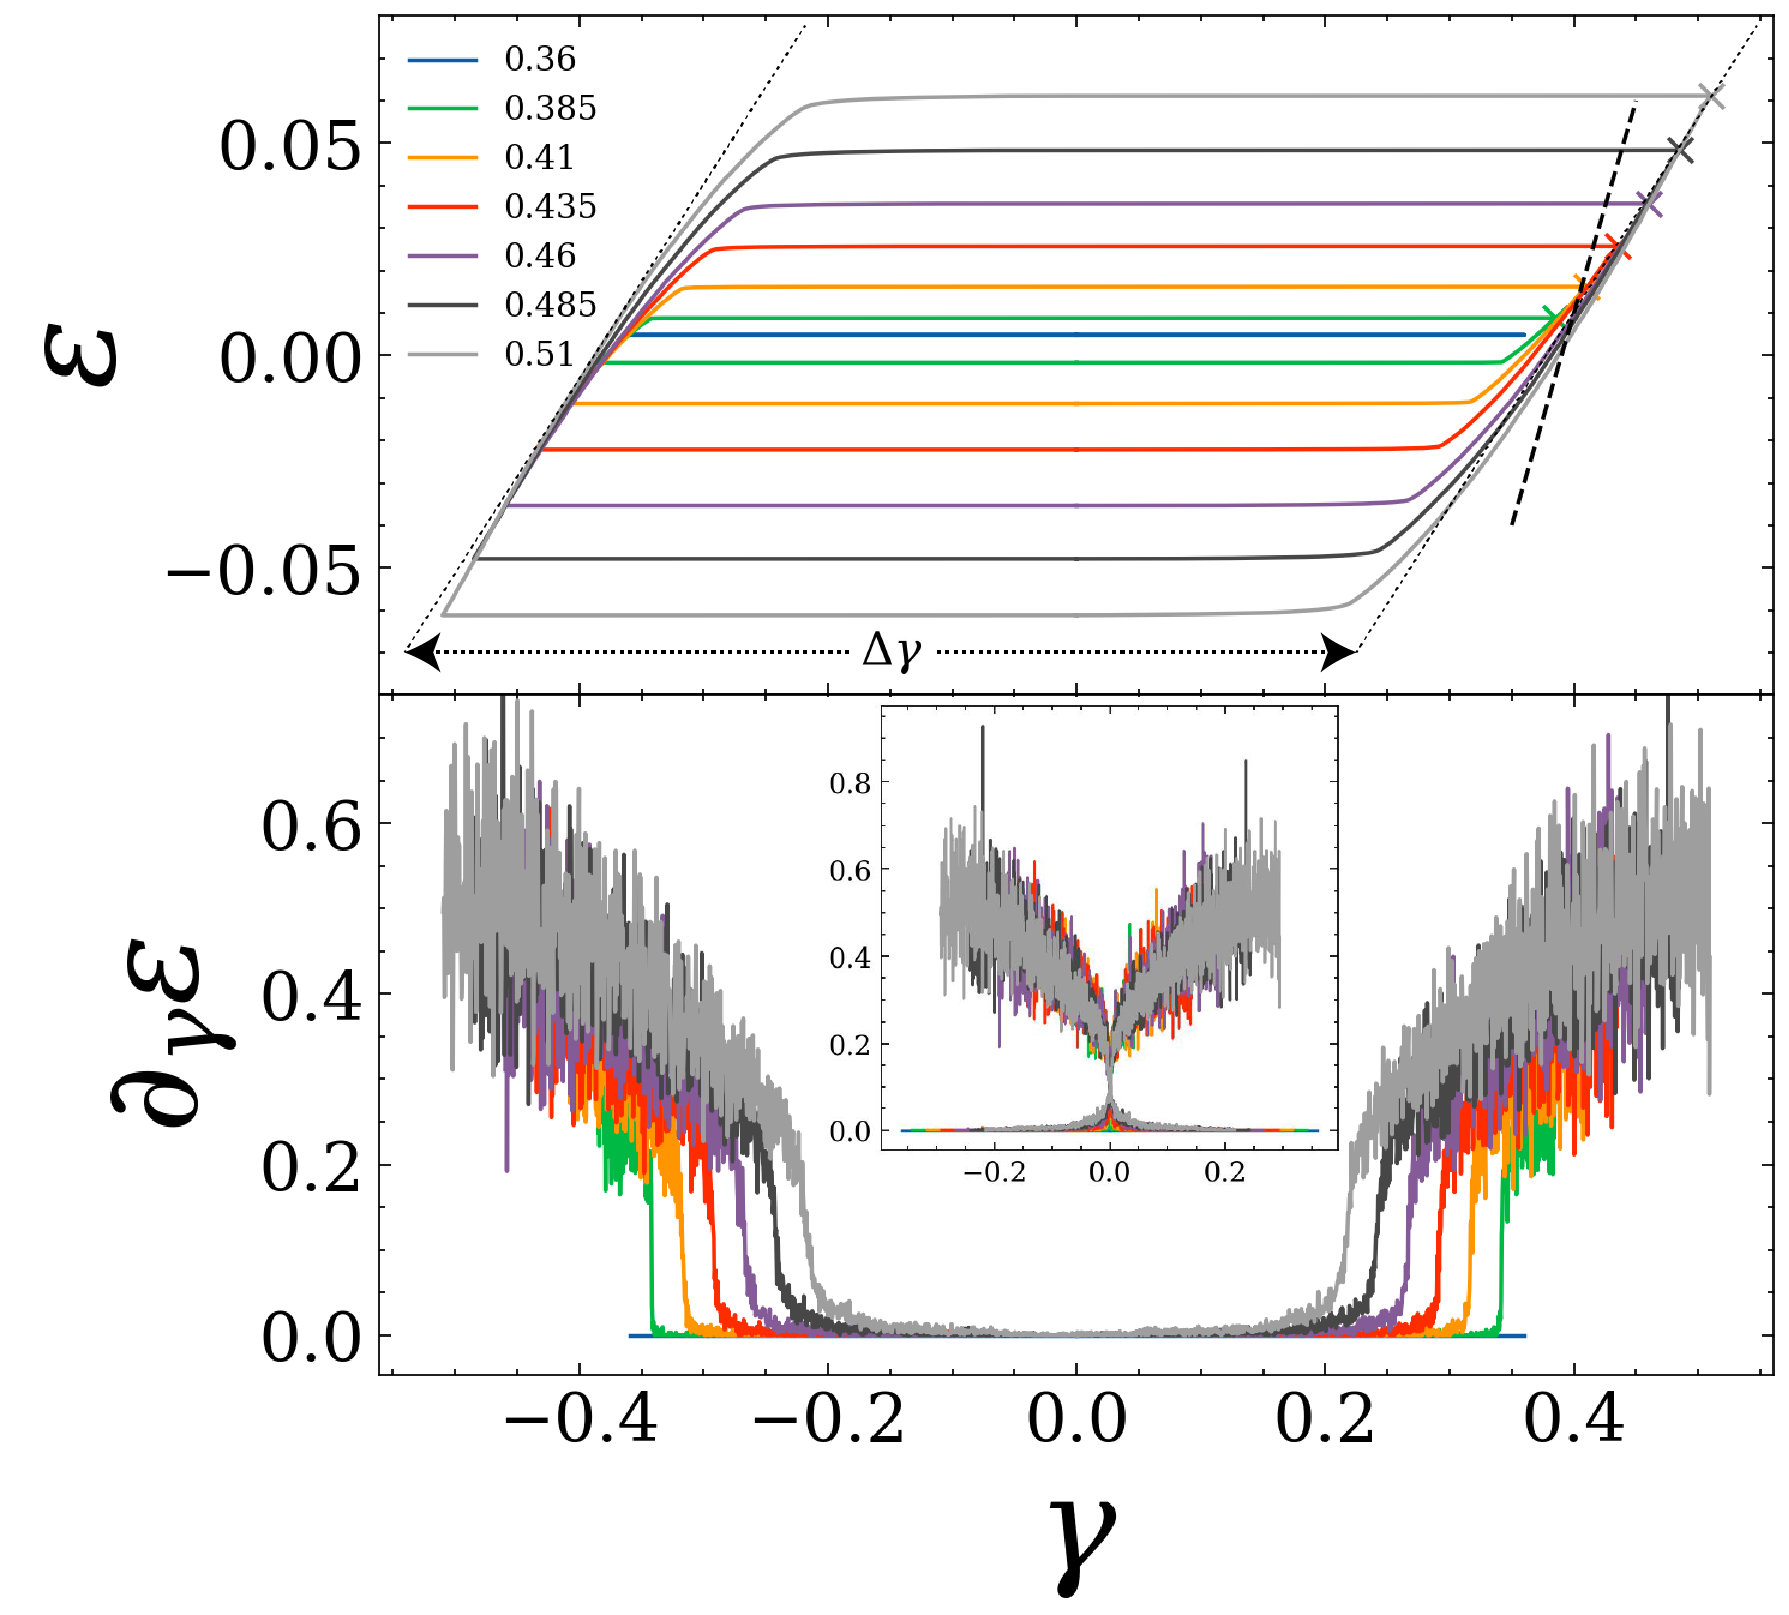
\includegraphics[width = 1.\columnwidth]{fig_epsilon_vs_Gamma.png}%
\caption{Plastic strain $\varepsilon$ (ensemble average) vs. strain $\gamma$ for different strain amplitudes (color online) in the steady state. The dashed line is an eye guide with a slope of unity.}
\end{figure}
%%%%%%%%%%%%%%%%%%%%%%%%%%%%%%%%%%%%%%%%%%%%%%%%%%%%%%%%%%%%%%%%%%%%%%

%%%%%%%%%%%%%%%%%%%%%%%%%%%%%%%% Figure 2 %%%%%%%%%%%%%%%%%%%%%%%%%%%%%
\begin{figure}[h!]
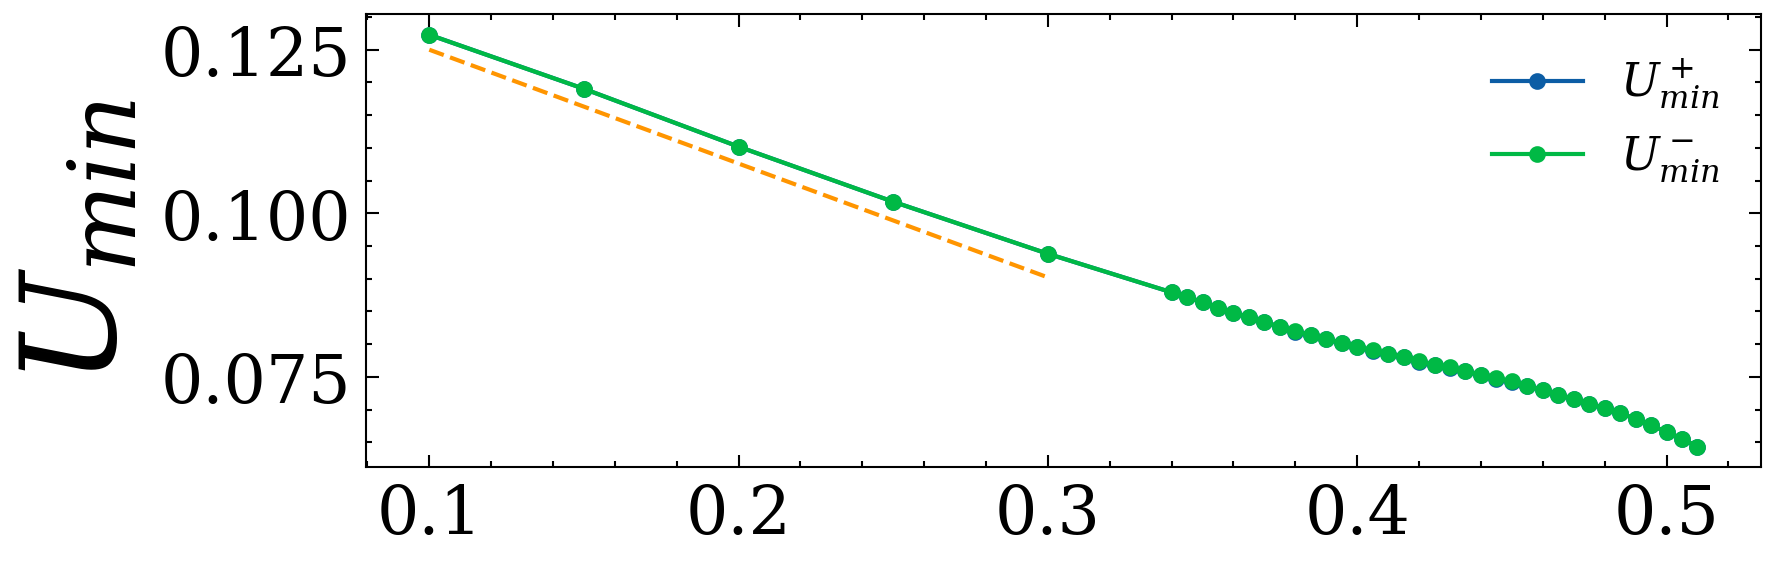
\includegraphics[width = 1.\columnwidth]{fig_Umin.png}%
\caption{The ground state energy $U_{min}$ vs $\gamma$ }
\end{figure}
%%%%%%%%%%%%%%%%%%%%%%%%%%%%%%%%%%%%%%%%%%%%%%%%%%%%%%%%%%%%%%%%%%%%%%

%%%%%%%%%%%%%%%%%%%%%%%%%%%%%%%% Figure 3 %%%%%%%%%%%%%%%%%%%%%%%%%%%%%
\begin{figure}[h!]
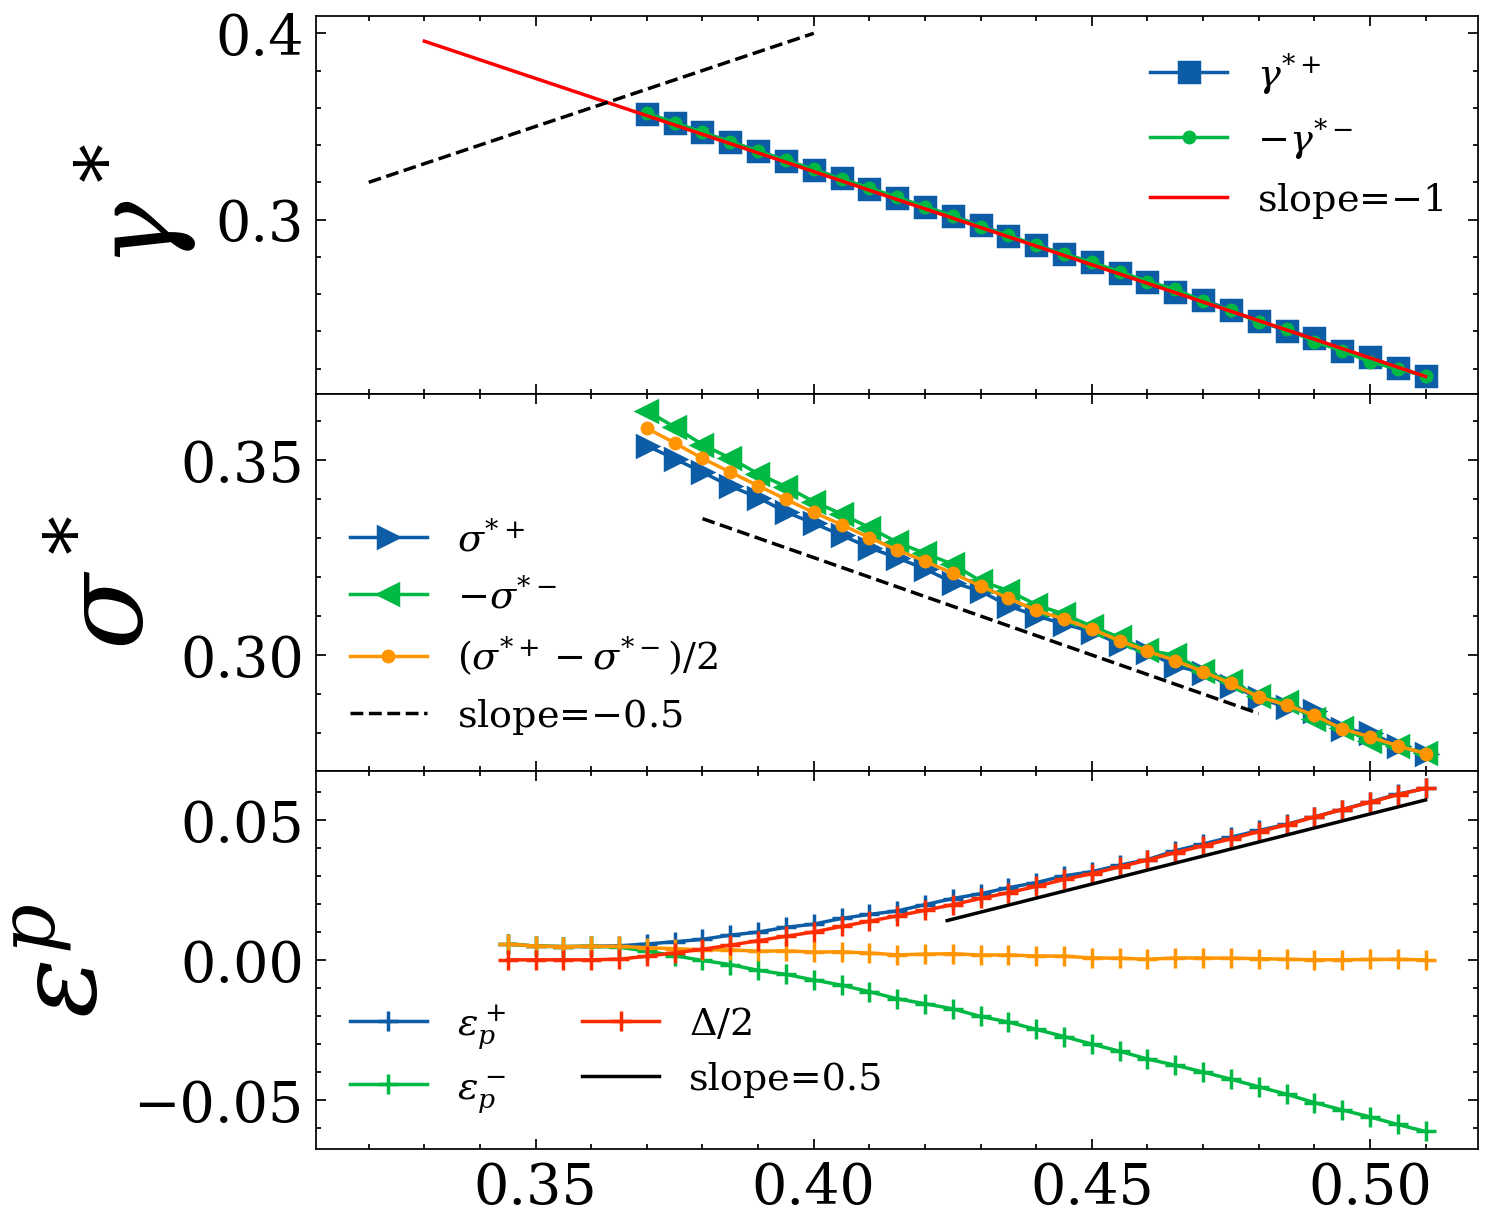
\includegraphics[width = 1.\columnwidth]{fig_gammastar_sigmastar_epsilonp_vs_Gamma.png}%
\caption{Top panel: the characteristic driving strain value $\gamma^*$ in the forward (blue) and the backward (green) sweep directions. Middle panel: the characteristic stress value $\sigma^*$ in the forward (blue) and the backward (green) sweep directions.Bottom panel: plastic strain plateau at the forward turning point $\varepsilon^+$ (blue) and at the backward turning point $\varepsilon^-$ (green). }
\end{figure}
%%%%%%%%%%%%%%%%%%%%%%%%%%%%%%%%%%%%%%%%%%%%%%%%%%%%%%%%%%%%%%%%%%%%%%
%%%%%%%%%%%%%%%%%%%%%%%%%%%%%%%% Figure 2 %%%%%%%%%%%%%%%%%%%%%%%%%%%%%
\begin{figure}[h!]
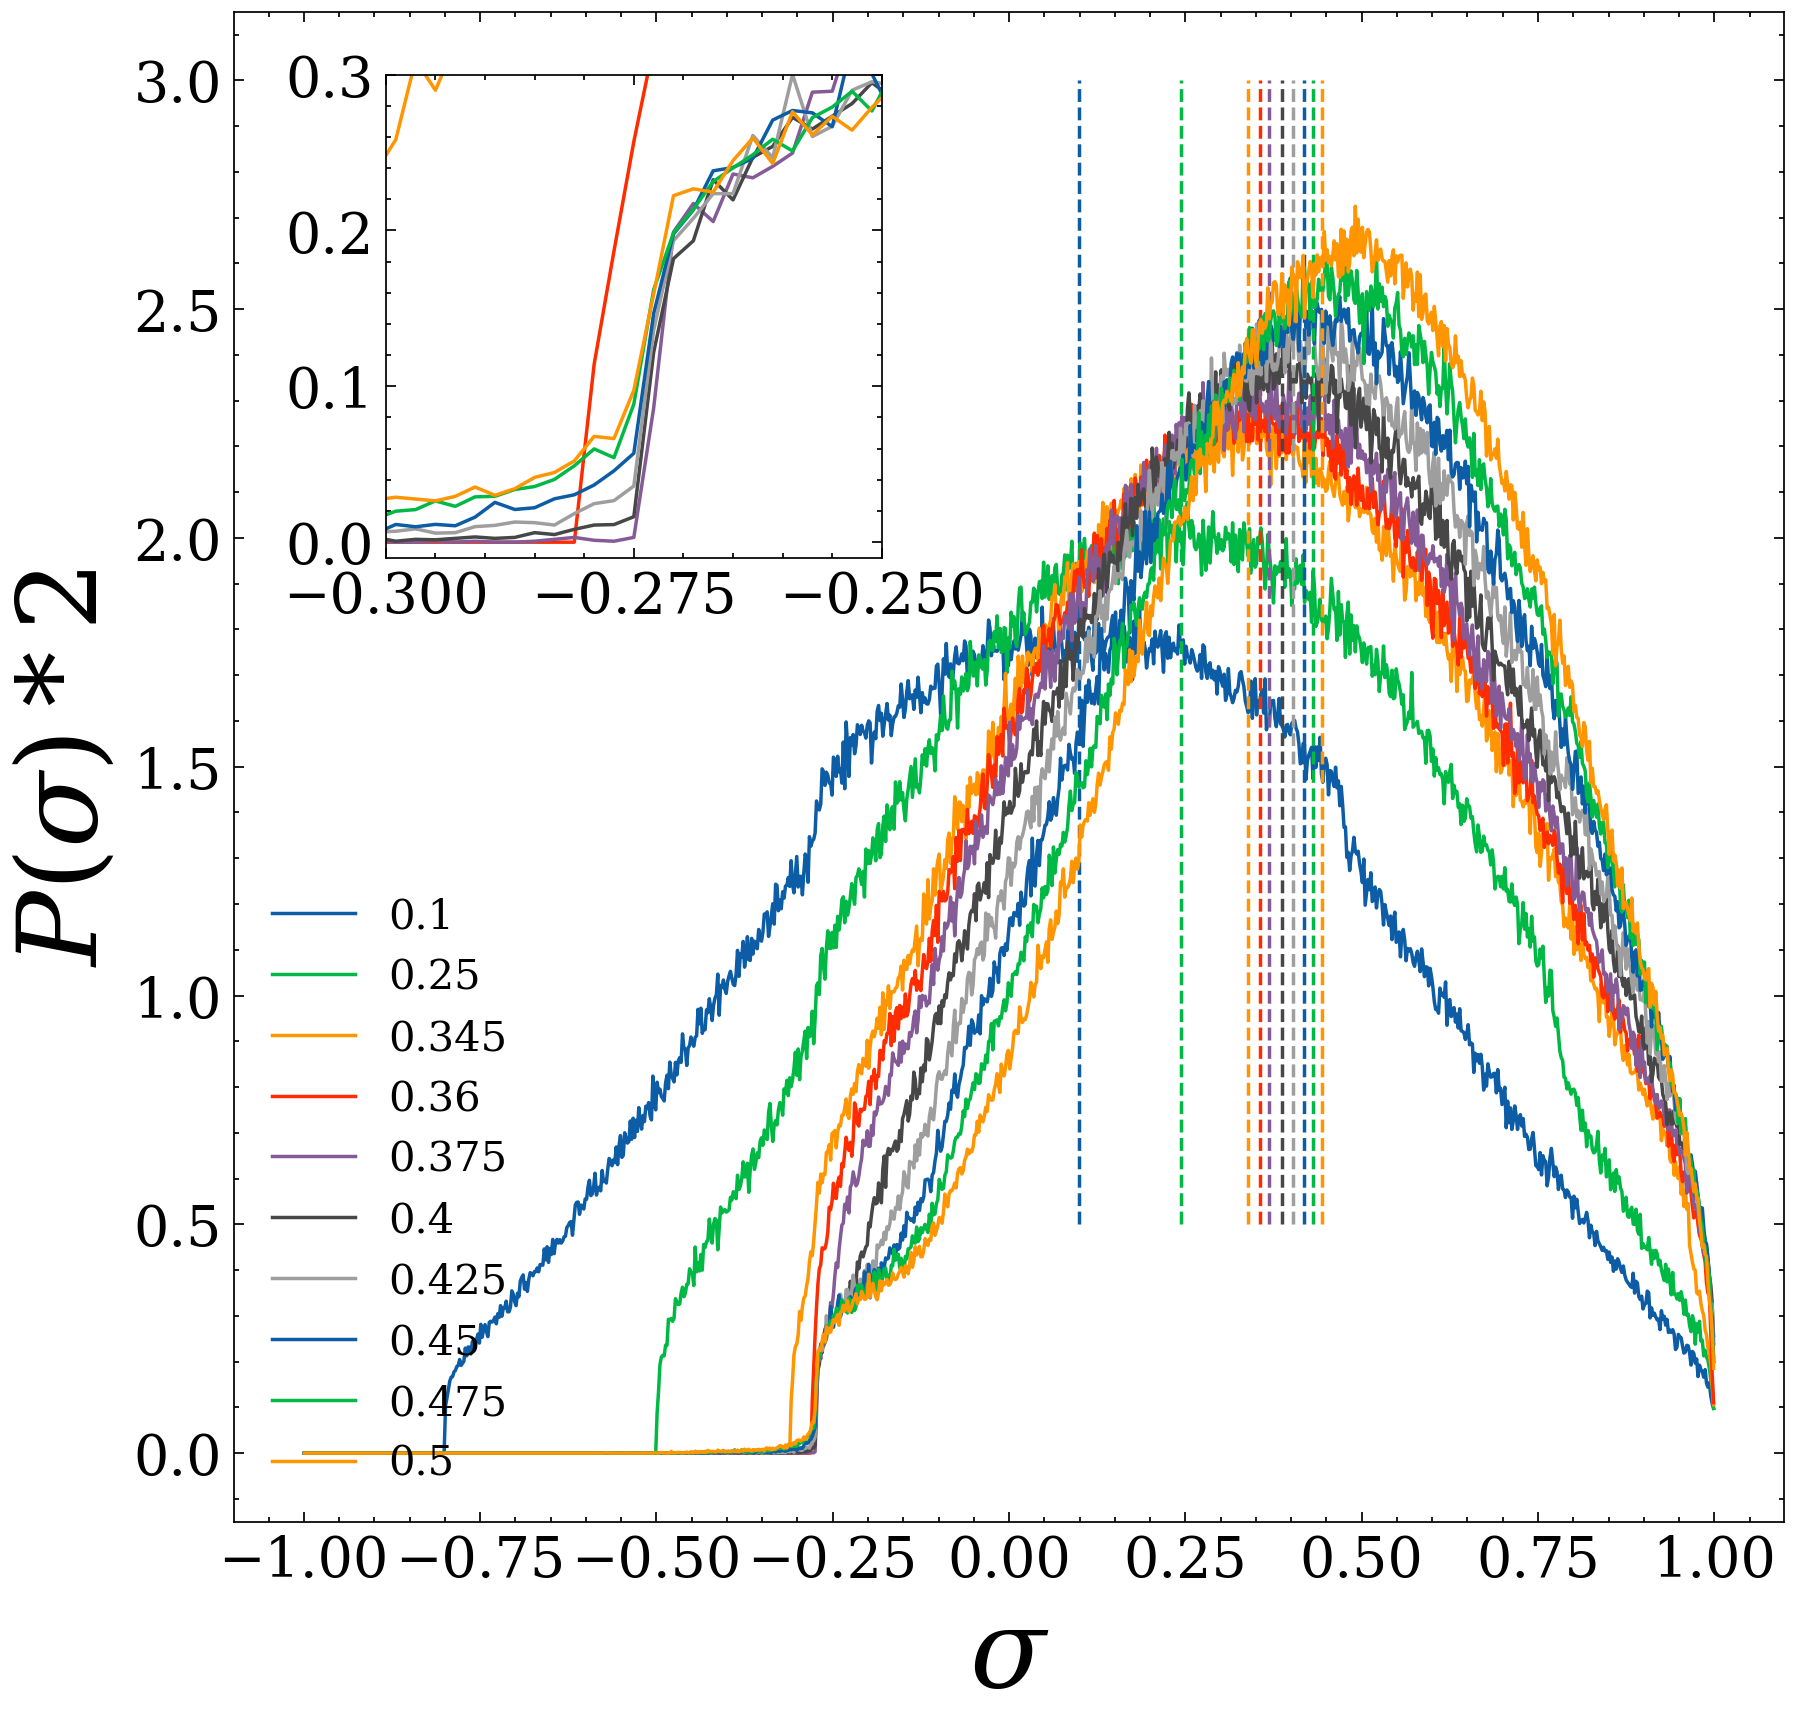
\includegraphics[width = 1.\columnwidth]{fig_P(sigma)_DepsilonDgamma.png}%
\caption{The distribution of the stress $\sigma$ at the forward turning point ($\gamma=\Gamma$) }
\end{figure}
%%%%%%%%%%%%%%%%%%%%%%%%%%%%%%%%%%%%%%%%%%%%%%%%%%%%%%%%%%%%%%%%%%%%%%


%%%%%%%%%%%%%%%%%%%%%%%%%%%%%%%% Figure 3 %%%%%%%%%%%%%%%%%%%%%%%%%%%%%
% \begin{figure}[h!]
% \includegraphics[width = 1.\columnwidth]{figure_3.png}%
% \caption{Logarithmic derivative of $\varepsilon_p$ w/r/t/ $gamma$. $d[log(\varepsilon_p)]/d[\log(\gamma)]$ vs. $\gamma$. [updated] }
% \end{figure}
% %%%%%%%%%%%%%%%%%%%%%%%%%%%%%%%%%%%%%%%%%%%%%%%%%%%%%%%%%%%%%%%%%%%%%%
% %%%%%%%%%%%%%%%%%%%%%%%%%%%%%%%% Figure 4 %%%%%%%%%%%%%%%%%%%%%%%%%%%%%
% \begin{figure}[h!]
% \includegraphics[width = 1.\columnwidth]{to_do_list_1/activity_vs_amp_1.png}%
% \caption{$\gamma^*$ vs. amplitude [updated]}
% \end{figure}
% %%%%%%%%%%%%%%%%%%%%%%%%%%%%%%%%%%%%%%%%%%%%%%%%%%%%%%%%%%%%%%%%%%%%%%
% %%%%%%%%%%%%%%%%%%%%%%%%%%%%%%%% Figure 5 %%%%%%%%%%%%%%%%%%%%%%%%%%%%%
% \begin{figure}[h!]
% \includegraphics[width = 1.\columnwidth]{to_do_list_1/activity_vs_amp_1.png}%
% \caption{$\sigma^*$ vs. amplitude [updated]}
% \end{figure}
% %%%%%%%%%%%%%%%%%%%%%%%%%%%%%%%%%%%%%%%%%%%%%%%%%%%%%%%%%%%%%%%%%%%%%%

% %%%%%%%%%%%%%%%%%%%%%%%%%%%%%%%% Figure 6 %%%%%%%%%%%%%%%%%%%%%%%%%%%%%
% \begin{figure}[h!]
% \includegraphics[width = 1.\columnwidth]{to_do_list_1/activity_vs_amp_1.png}%
% \caption{$\gamma_{min}$ vs. amplitude [updated]}
% \end{figure}
% %%%%%%%%%%%%%%%%%%%%%%%%%%%%%%%%%%%%%%%%%%%%%%%%%%%%%%%%%%%%%%%%%%%%%%

% %%%%%%%%%%%%%%%%%%%%%%%%%%%%%%%% Figure 7 %%%%%%%%%%%%%%%%%%%%%%%%%%%%%
% \begin{figure}[h!]
% \includegraphics[width = 1.\columnwidth]{to_do_list_1/activity_vs_amp_1.png}%
% \caption{$\sigma_{min}$ vs. amplitude [new]}
% \end{figure}
% %%%%%%%%%%%%%%%%%%%%%%%%%%%%%%%%%%%%%%%%%%%%%%%%%%%%%%%%%%%%%%%%%%%%%%

% % %%%%%%%%%%%%%%%%%%%%%%%%%%%%%%%% Figure 8 %%%%%%%%%%%%%%%%%%%%%%%%%%%%%
% % \begin{figure}[h!]
% % \includegraphics[width = 1.\columnwidth]{to_do_list_1/activity_vs_amp_1.png}%
% % \caption{$U_{min}$ vs. amplitude [updated]}
% % \end{figure}
% % %%%%%%%%%%%%%%%%%%%%%%%%%%%%%%%%%%%%%%%%%%%%%%%%%%%%%%%%%%%%%%%%%%%%%%

% %%%%%%%%%%%%%%%%%%%%%%%%%%%%%%%% Figure 9 %%%%%%%%%%%%%%%%%%%%%%%%%%%%%
% \begin{figure}[h!]
% \includegraphics[width = 1.\columnwidth]{to_do_list_1/activity_vs_amp_1.png}%
% \caption{Global period distribution [updated]}
% \end{figure}
% %%%%%%%%%%%%%%%%%%%%%%%%%%%%%%%%%%%%%%%%%%%%%%%%%%%%%%%%%%%%%%%%%%%%%%

% %%%%%%%%%%%%%%%%%%%%%%%%%%%%%%%% Figure 10 %%%%%%%%%%%%%%%%%%%%%%%%%%%%%
% \begin{figure}[h!]
% \includegraphics[width = 1.\columnwidth]{to_do_list_1/activity_vs_amp_1.png}%
% \caption{Average global period [new]}

% \end{figure}
% %%%%%%%%%%%%%%%%%%%%%%%%%%%%%%%%%%%%%%%%%%%%%%%%%%%%%%%%%%%%%%%%%%%%%%

% %%%%%%%%%%%%%%%%%%%%%%%%%%%%%%%% Figure 11 %%%%%%%%%%%%%%%%%%%%%%%%%%%%%
% \begin{figure}[h!]
% \includegraphics[width = 1.\columnwidth]{to_do_list_1/activity_vs_amp_1.png}%
% \caption{Distribution of limit cycles [updated]}
% \end{figure}
% %%%%%%%%%%%%%%%%%%%%%%%%%%%%%%%%%%%%%%%%%%%%%%%%%%%%%%%%%%%%%%%%%%%%%%

% %%%%%%%%%%%%%%%%%%%%%%%%%%%%%%%% Figure 12 %%%%%%%%%%%%%%%%%%%%%%%%%%%%%
% \begin{figure}[h!]
% \includegraphics[width = 1.\columnwidth]{to_do_list_1/activity_vs_amp_1.png}%
% \caption{Total dissipated energy per cycle [new]}
% \end{figure}
% %%%%%%%%%%%%%%%%%%%%%%%%%%%%%%%%%%%%%%%%%%%%%%%%%%%%%%%%%%%%%%%%%%%%%%


% %%%%%%%%%%%%%%%%%%%%%%%%%%%%%%%% Figure 13 %%%%%%%%%%%%%%%%%%%%%%%%%%%%%
% \begin{figure}[h!]
% \includegraphics[width = 1.\columnwidth]{to_do_list_1/activity_vs_amp_1.png}%
% \caption{Total activity per cycle [new]}
% \end{figure}
% %%%%%%%%%%%%%%%%%%%%%%%%%%%%%%%%%%%%%%%%%%%%%%%%%%%%%%%%%%%%%%%%%%%%%%


% \subsection{}
% \subsubsection{}

% If in two-column mode, this environment will change to single-column format so that long equations can be displayed. 
% Use only when necessary.
%\begin{widetext}
%$$\mbox{put long equation here}$$
%\end{widetext}

% Figures should be put into the text as floats. 
% Use the graphics or graphicx packages (distributed with LaTeX2e).
% See the LaTeX Graphics Companion by Michel Goosens, Sebastian Rahtz, and Frank Mittelbach for examples. 
%
% Here is an example of the general form of a figure:
% Fill in the caption in the braces of the \caption{} command. 
% Put the label that you will use with \ref{} command in the braces of the \label{} command.
%
% \begin{figure}
% \includegraphics{}%
% \caption{\label{}}%
% \end{figure}

% Tables may be be put in the text as floats.
% Here is an example of the general form of a table:
% Fill in the caption in the braces of the \caption{} command. Put the label
% that you will use with \ref{} command in the braces of the \label{} command.
% Insert the column specifiers (l, r, c, d, etc.) in the empty braces of the
% \begin{tabular}{} command.
%
% \begin{table}
% \caption{\label{} }
% \begin{tabular}{}
% \end{tabular}
% \end{table}

% If you have acknowledgments, this puts in the proper section head.
%\begin{acknowledgments}
% Put your acknowledgments here.
%\end{acknowledgments}

% Create the reference section using BibTeX:
% \bibliography{your-bib-file}

\end{document}
%
% ****** End of file aiptemplate.tex ******